\documentclass[a4paper,11pt]{article}
\usepackage[american]{babel}
\usepackage{hyperref}
\usepackage{geometry}
\usepackage{sectsty}
\usepackage[table,svgnames]{xcolor}
\usepackage{graphicx}
\usepackage{listings}
\usepackage[T1]{fontenc}
\usepackage[utf8]{inputenc}
\usepackage{mathptmx}

\newcommand{\authortitle}{Priv.-Doz.~Dr.~Ing.}
\newcommand{\authorname}{Martin Lambers}
\newcommand{\course}{Rendering}
\newcommand{\tutorial}{Tutorial 9}

\hypersetup{
  colorlinks = true,
  urlcolor = blue,
  citecolor = blue,
  pdfauthor = {\authorname},
  pdftitle = {\course{} \tutorial},
  pdfsubject = {\course Tutorial},
  pdfpagemode = UseNone
}

\geometry{
  body={6.6in, 8.5in},
  left=1.0in,
  top=1.25in
}

% Custom section fonts
\sectionfont{\rmfamily\mdseries\Large}
\subsectionfont{\rmfamily\mdseries\large}
\subsubsectionfont{\rmfamily\mdseries\normalsize}
\paragraphfont{\rmfamily\mdseries\itshape\normalsize}

% Don't indent paragraphs; leave space instead
\setlength\parindent{0em}
\setlength\parskip{.5\baselineskip plus .5\baselineskip}

% In-text code sample
\newcommand{\code}[1]{\texttt{#1}}
% Larger code examples with lstlisting
\definecolor{cgblue}{rgb}{0.2,0.2,0.7}
\lstloadlanguages{C}
\lstdefinelanguage[OpenGL]{C}[ANSI]{C}{%
    morekeywords={bool,bvec2,bvec3,bvec4,ivec2,ivec3,ivec4,vec2,vec3,vec4}
}
\lstset{%
    language=[OpenGL]C,
    basicstyle=\footnotesize\ttfamily,%
    keywordstyle=\color{cgblue},%
    directivestyle=\color{cgblue},%
    identifierstyle=,%
    commentstyle=\color{cgblue!50!white}\itshape,%
    stringstyle=\color{cgblue!80!white},%
    numbers=none,%
    numberstyle=\tiny,%
    extendedchars=true,%
    showspaces=false,%
    showstringspaces=false,%
    showtabs=false,%
    breaklines=false,%
    frame=single,%
    frameround=tttt,%
    backgroundcolor=\color{white},%
    literate={\\\%}{\%}1,
    escapechar=\%
}


\begin{document}

\thispagestyle{empty}

\LARGE

\centerline{\course{} \tutorial}

\vspace{1ex}

\normalsize

\centerline{\authortitle{} \authorname}

%\vspace{.5\baselineskip}

\section*{Assigment 1}

Use a fractal combination of Worley noise values to create a ``crumpled paper''
effect:

$\displaystyle G_1(u,v) = \sum_{i=0}^{N} \frac{1}{2^i}F_1(2^i(u,v))$

The result should look like the image on the left below when used as
a texture.

What is the cause of the line artifacts you see? How can they be fixed?
If you find the right answer, the result should look like the middle image
below.

Of course the crumple effect is not intended to be used as a texture directly.
Instead, it is better interpreted as a bump map. Create a normal map from it
using the function \code{bumpMapToNormalMap()} from \code{import.hpp}, with a
bump factor of 16 and a virtual size of $256\times 256$ as parameters (as a
starting point; feel free to experiment).

The result might look similar to the image on the right below.

A basic implementation of Worley noise is included in the tutorial material,
together with the example scene.

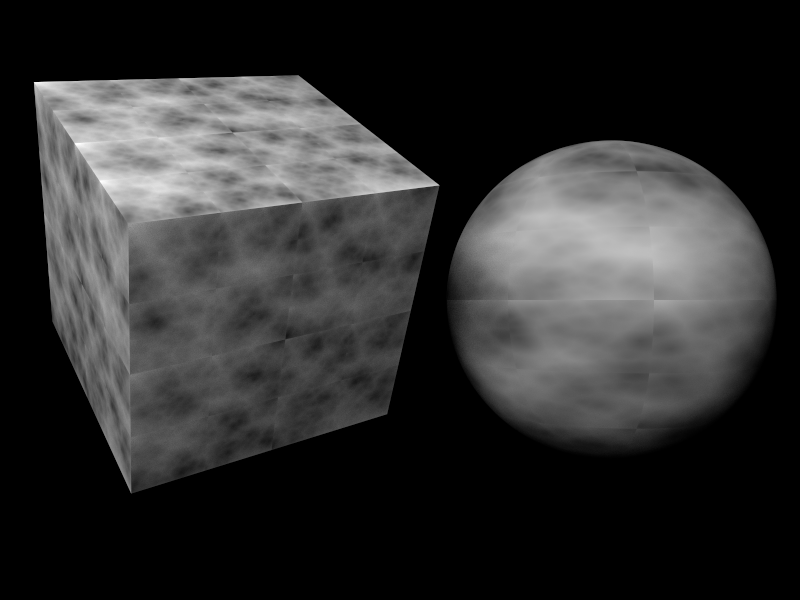
\includegraphics[width=.32\textwidth]{./fig/09-result-with-artifacts.png}\hfill
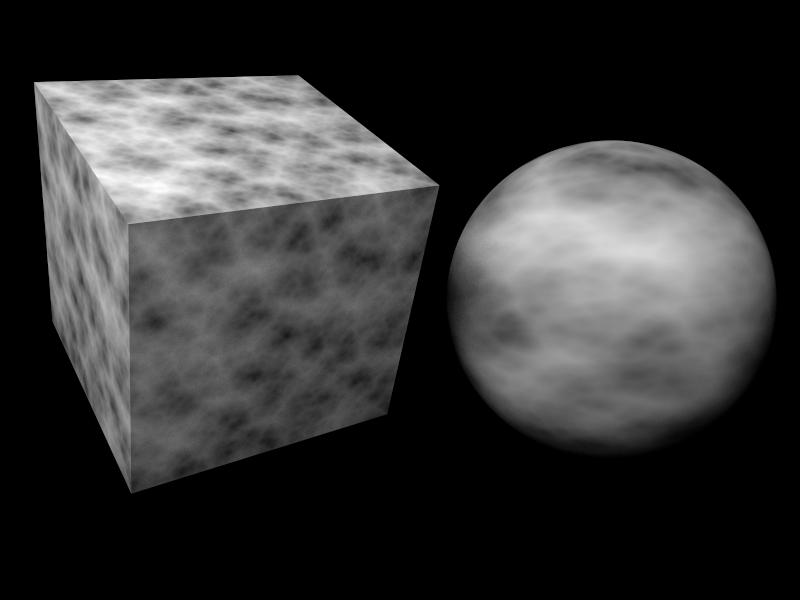
\includegraphics[width=.32\textwidth]{./fig/09-result-without-artifacts.png}\hfill
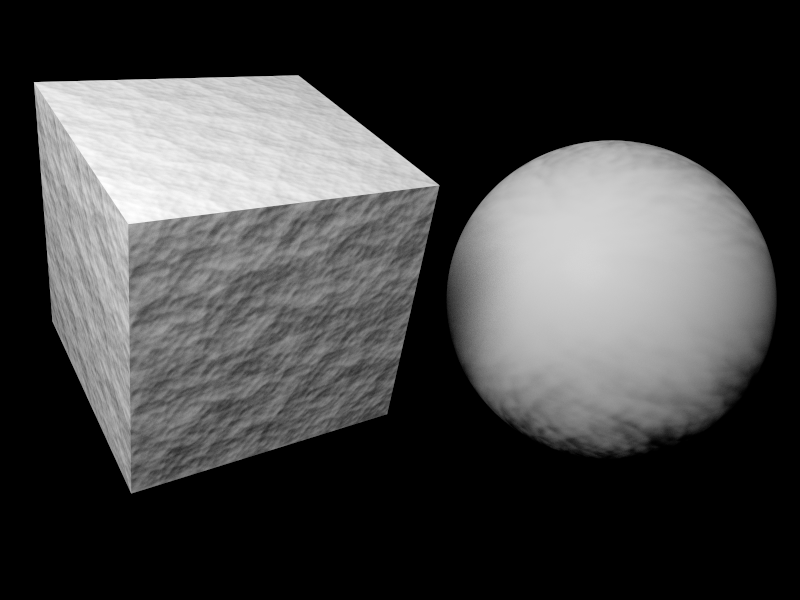
\includegraphics[width=.32\textwidth]{./fig/09-result-as-bumpmap.png}

\end{document}
